\comment{
Typical DDMS workloads require large state, necessitating the use of
suitable storage techniques. Compared to traditional DBMS with
primarily ad-hoc query workloads, DDMS have more
information to use when constructing a task-specific storage solution.
} % end comment


We now examine two components of DBToaster's solution to storage in a DDMS: (1)
The DBToaster compiler produces data structures designed specifically for the
compiled DDMS' target query workload. (2) By analyzing the patterns with which
data is accessed, DBToaster constructs a data layout strategy (for pages on a
disk, servers in a cluster, etc.) that limits IO overhead.

\noindent
{\bf Data structures}.
%
DBToaster uses multi-key (i.e.,
multi-dimensional) maps to represent materialized views. The generated code
performs lookups of slices of the maps, using partial keys, fixing some
dimensions and iterating over the others. Recall the right-hand side of line 2
in the code listing in Section~\ref{sec:compilation}. This is a partial lookup
on map $m\_c$ with only {\tt ck} defined by the trigger arguments.
%
In addition to exact and partial lookups, DBToaster maps support
range lookups by inequality predicates.

\comment{
Regardless of whether data is stored in memory, on disk, or across an entire
cluster, efficient disk access begins with good representation.  As its data
storage primitive, DBToaster uses multi-key maps, which have thus far not been
formally defined.

Fundamentally, a multi-key map is a simple key-value store with structured
(i.e., schema-defined) keys and values, as well as some iteration capabilities. 
However, generated statements do not typically iterate over the entire
datastructure.  In the common case, statements iterate over keys matching a
selection predicate.  For example, when updating Section \ref{sec:dbtoaster}'s
$m\_c$ after an insertion into \texttt{lineitem}, we iterate over all values
matching the predicate \texttt{@ok = orderkey}.

Though similar to relational tables in this respect, there are two subtle, but
critical differences: (1) The map's value at each point is defined not by the
data stored in it, but rather as a function (subquery) over the state of the
database.  (2) Unlike a relational table, where absent keys imply NULL values,
multi-key maps are defined for all keys conforming to the map's schema.

These two differences are closely related.  A map's value must be defined for
all keys, because all updates are specified as deltas.  In the absence of prior
state, this value can be derived from lower level maps, or the base relations. 
Interestingly, for non-nested queries without inequalities, this value always
begins at zero.  So long as the maps are maintained incrementally, we never need
to compute the initial value.

This functional view of maps paves the way for a range of entirely different
data representations: 
}

In their simplest form, out-of-core maps are implemented by a simple
relational-style key-value store with secondary indices~\cite{berkeleydb}.
\comment{
However, the map could simply act as an incrementally maintained cache.
Recently computed values are not only available for re-use, they are dynamically
updated as the underlying function gets new inputs.
}
Inequality predicates, and aggregations including such predicates, are
implemented efficiently using maps that store cumulative
sums~\cite{rangequeries}.  Maps can apply compression techniques to address
frequently repeating data.
\comment{
As another example, a probabilistic database built on top of a DDMS might use
maps representing regressions, a markov random field, a bayes nets, etc\ldots
}
DBToaster customizes the data structures backing each materialized view based
on statement-level information on accesses, applying static compile-time
techniques to construct specialized data structures.

With substantial specialization of data structures as part of compiling
transitions, DBToaster is free to consider a range of runtime issues in data
structure tuning and adaptation, including how to best perform fine-grained
operations such as incremental and partial
indexing~\cite{stonebreaker-sigrec:89}. The key challenge to be addressed is how
to provide data structures with a low practical update cost (avoiding expensive
index rebalancing and hash-table rebucketing) while gradually ensuring the
lookup requirements of our data structures are retained over time, amortizing
data structure construction with continuous query execution.


\noindent
{\bf Partitioning and co-clustering by data flow analysis}.
%
Database partitioning and co-clustering decisions
are traditionally made based on a combination of
(a) workload statistics, (b) information on schema and integrity constraints
(such as key-foreign key constraints, a popular basis for co-clustering
decisions), and (c) a body of expert insights into how databases execute
queries. Ideally, such decisions should be based on a combination
of (a), (b), and a {\em data flow analysis}\/ of the system's query execution code,
instantiated with the query plan, or view maintenance code. In classical
DBMS however, this is too difficult to be practical.

Fortunately, data flow analysis turns out to be feasible for compiled DDMS
transition programs: in fact, it is rather easy. A transition program statement
reads from several maps and writes to one, prescribing dependencies between
those maps occurring on the right-hand side of the statement (reading), and the
one on the left-hand side (writing). As pointed out in Section
\ref{sec:dbtoaster}, transition program statements admit a perfectly
data-parallel implementation: consequently, a statement never imposes a
dependency between two items of the same map and any horizontal partitioning
across the involved maps map keeps updates strictly local.
%
Using these data flow dependencies, partitioning and co-clustering
decisions can be made by
% assigning a data statistics-dependent cost to placing dependent data
%in different partitions and
solving a straightforward min-cut style optimization problem.



\comment{
Even with good data structures, haphazard data placement leads to poor
performance.  Though precise workload data may not be available at compile time,
DBToaster optimizes the way it lays out its database across memory, a disk, or
even a server cluster, based on the query workload it is constructed with.


The following notion of a \textit{messaging graph} is an abstraction for
doing this:
A transition function is represented as a bipartite directed hypergraph;
nodes on the left represent portions of the database being read from, nodes on
the right represent a portions being written to, and each hyperedge represents
an independent subtask of the transition function.  An example is shown in
Figure \ref{fig:diag:messagingGraph}a.

\begin{figure}
\begin{center}
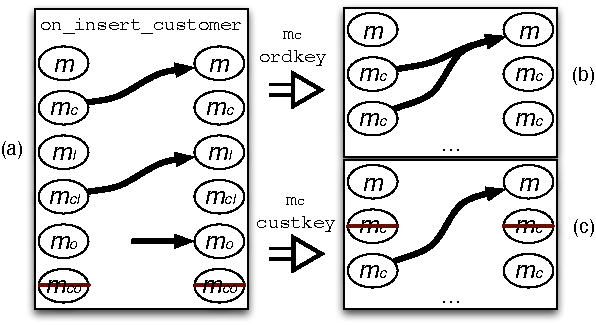
\includegraphics[width=2.5in]{graphics/MessagingGraph}
\end{center}

\vspace{-6mm}

\caption{An example of a messaging graph based on Section \ref{sec:dbtoaster}'s example query.  (a) The messaging graph for the \texttt{on\_insert\_customer} event.  (b) The effects of splitting view $m\_c$ on \texttt{ordkey}.  (c) The effects of splitting $m\_c$ on \texttt{custkey}.}
\label{fig:diag:messagingGraph}
\vspace*{-0.2in}
\end{figure}

For example, consider the transition function that results from an update to the
customer table.  One specific subtask of this transition reads $m\_c$ and writes
to $m$.  Treating each view as a node, this task has one edge with one read node
and one write node.

DBToaster considers database layout in terms of how it partitions data across a
physical medium (i.e., memory, disk pages, or a cluster).  Viewed through the
messaging graph, a partitioning is an assignment of all nodes in the graph to
one (or more, in the case of replication) partition.  For example, if they were
small enough, $m$ and $m\_c$ might be placed on one disk page each.  Thus, the
subtask requires a read on one page, and an update to a second.

Subdivision of individual views is represented in the messaging graph by
splitting of graph nodes.  Of particular interest is how the new nodes interact
with the hyperedge(s) connected to the original node.  As the split occurs, a
node may stay connected to a hyperedge, the hyperedge may likewise be split, or
in some cases, only one node will remain connected (see Figure
\ref{fig:diag:messagingGraph}b,c).  DBToaster can exploit the limited range of
node split/hyperedge interactions to select an effective partitioning scheme.

For example, when partitioning $m\_c$, horizontal partitioning on the value of
\texttt{ordkey} increases the number of nodes connected to the
\texttt{on\_insert\_customer} task edge, while using \texttt{custkey} does not
provoke an increase.  If the data represented by these nodes is split across
multiple disks or servers, the computation must still access all of them.  The
roles are reversed for the \texttt{on\_insert\_order} task edge.  Under (the
false) assumption that both insert events occur with identical frequency,
DBToaster can partition on both keys to minimize the number of connected nodes.

Additional knowledge about the dataset enhances the messaging graph produced by
DBToaster.  For instance, the ER diagram can be integrated into the messaging
graph; the chain of foreign key dependencies in $q$ is strictly hierarchical. 
DBToaster uses this information and creates partitions along a single axis with
a secondary index to bound the number of partitions accessed by each update
subtask, with respect to the total number of partitions generated.  Similarly,
this information is used by DBToaster to select a partitioning scheme that
places nodes typically connected by a subtask into a single partition; this is
analogous to co-clustering in a traditional DBMS.

} % end comment
